
\documentclass[12pt,a4paper]{article}
\usepackage[utf8]{inputenc}
\usepackage[T1]{fontenc}
\usepackage[brazil]{babel}
\usepackage{amsmath,amssymb,amsfonts}
\usepackage{graphicx}
\usepackage{booktabs}
\usepackage{hyperref}
\usepackage{minted}
\usepackage{tocloft}
\usepackage{geometry}
\usepackage{csvsimple}
\geometry{margin=2.5cm}
\usepackage{wrapfig} % In your preamble

% Minted + suporte a quebras de linha e página
\usepackage{minted}
\usepackage{fvextra} % extensão para verbatim/minted

% Configurações globais do minted
\setminted{
    breaklines=true,        % quebra de linha automática
    breakanywhere=true,     % pode quebrar em qualquer ponto
    fontsize=\small,
    autogobble=true,        % remove indentação comum
    breaksymbolleft={},     % sem símbolos feios nas quebras
    breaksymbolright={},
}

\usepackage{siunitx}
\sisetup{
  round-mode=places,
  round-precision=9,
  table-number-alignment=center,
  detect-all,
  scientific-notation=true
}

\title{PCS5029/PTC5725 -- Aula 06\\\large Introdução aos Métodos Espectrais}
\author{Renan de Luca Avila}
\date{\today}

\begin{document}
\begin{titlepage}
\centering

\includegraphics[width=0.35\textwidth]{EP.jpg}\par\vspace{1cm}
{\scshape\LARGE Escola Politécnica da Universidade de São Paulo\par}
\vspace{1.5cm}
{\huge\bfseries Aula 09 -- Métodos Espectrais\par}
\vspace{0.5cm}
{\Large Resolução da tarefa\par}
\vfill
{\large Renan de Luca Avila\par}
{\large \today\par}
\end{titlepage}

\tableofcontents
\newpage

\section{Resumo}
Este relatório implementa, em Python, os exercícios apresentados nos slides da Aula 09 (Prof.\ Osvaldo Guimarães), e discute as soluções. O documento contém códigos completos, figuras e tabelas, além de apêndices com setup e fontes.

% \subsection{Exercício X}

% \subsubsection{Enunciado}
% % Descreva o enunciado aqui com os detalhes matemáticos

% \subsubsection{Planejamento e fundamentos teóricos}
% % Descreva o plano para resolver o problema e cite os fundamentos teóricos que sustentam o plano, incluindo fórmulas e equações justificando o caminho escolhido

% \subsubsection{Etapas de implementação e funções principais}
% % Coloque citações de trechos do código aqui e explique o que cada uma delas faz relacionando com os fundamentos teóricos (use minted copiando trechos de código diretamente). Coloque trechos e os explique um a um, não coloque o código completo, pois este estará no apêndice referenciando o arquivo na pasta /code.

% \subsubsection{Resultados e discussão}
% % Coloque aqui figuras (da pasta /figures) e tabelas (da pasta /tables) que mostrem os resultados obtidos como saída do código e interprete os resultados

% \subsubsection{Conclusão}
% % Resuma o que fizemos para resolver e conclua com avaliações dos resultado

\section{Equação de Poisson Bidimensional com Pontos de Chebyshev--Lobatto}

Esta tarefa corresponde ao estudo apresentado no \textbf{slide 19 da Aula 09}, cujo objetivo é traduzir para \texttt{Julia} o código MATLAB do livro \emph{Spectral Methods in MATLAB} (Trefethen, 2000), especificamente o \textbf{Programa 16 --- página 70}, que resolve numericamente a equação de Poisson em duas dimensões utilizando o método espectral de Chebyshev.

O problema considerado é:

\begin{equation}
\Delta F(x,y)
=
10 \,\sin\!\big( 8x(y-1) \big),
\qquad (x,y)\in[-1,1]^2,
\end{equation}

sujeito à condição de contorno homogênea:

\[
F = 0 \quad \text{em todo o contorno}.
\]

Nosso objetivo é reproduzir fielmente, em Julia, o método numérico utilizado no código MATLAB original, analisar a solução obtida e estudar a influência do número de pontos de discretização.

\subsection{Citação dos códigos MATLAB originais}

A implementação MATLAB utilizada como referência é apresentada no livro \emph{Spectral Methods in MATLAB}, de Lloyd N. Trefethen, e consiste de dois blocos principais:

\begin{enumerate}
    \item A função que gera os pontos de Chebyshev–Lobatto e a matriz de diferenciação:
\end{enumerate}

\begin{minted}[fontsize=\small]{matlab}
% CHEB  compute D = differentiation matrix, x = Chebyshev grid
function [D,x] = cheb(N)
  if N==0, D=0; x=1; return, end
  x = cos(pi*(0:N)/N)'; 
  c = [2; ones(N-1,1); 2].*(-1).^(0:N)';
  X = repmat(x,1,N+1);
  dX = X-X';                  
  D  = (c*(1./c)')./(dX+(eye(N+1)));      % off-diagonal entries
  D  = D - diag(sum(D'));                 % diagonal entries
end
\end{minted}

\begin{enumerate}
    \item[2.] O programa principal que monta o operador Laplaciano via produto de Kronecker e resolve o sistema linear correspondente (\emph{Programa 16 – pág. 70 do livro}):
\end{enumerate}

\begin{minted}[fontsize=\small]{matlab}
% Poisson eq. on [-1,1]x[-1,1] with u=0 on boundary
N = 24; [D,x] = cheb(N); y = x;
[xx,yy] = meshgrid(x(2:N),y(2:N));
xx = xx(:); yy = yy(:);       % stretch 2D grids to 1D vectors
f = 10*sin(8*xx.*(yy-1));
D2 = D^2; D2 = D2(2:N,2:N); I = eye(N-1);
L = kron(I,D2) + kron(D2,I);  % Laplacian

u = L\f;                     % Solve system

uu = zeros(N+1,N+1);
uu(2:N,2:N) = reshape(u,N-1,N-1);
[xx,yy] = meshgrid(x,y);
value = uu(N/4+1,N/4+1);
\end{minted}

Esse código MATLAB constitui a \textbf{referência exata} a ser reproduzida em Julia, com fidelidade matemática e estrutural — adaptando apenas a sintaxe da linguagem e aproveitando as funcionalidades modernas do ecossistema Julia.

\subsection{Objetivos da Tarefa}

\begin{itemize}
    \item Reproduzir o método espectral de Trefethen utilizando \textbf{Chebyshev–Lobatto} para resolver a equação de Poisson 2D.
    \item Implementar em \texttt{Julia}, de forma modular e reutilizável, as seguintes rotinas:
    \begin{itemize}
        \item geração de pontos de Chebyshev–Lobatto;
        \item matriz de diferenciação $D$ e segunda derivada $D^2$;
        \item montagem do Laplaciano 2D via produto de Kronecker;
        \item solucionador genérico da equação de Poisson para diferentes funções $f(x,y)$.
    \end{itemize}
    \item Comparar o comportamento numérico da solução para diferentes discretizações:
    \[
    N = 12,\ 16,\ 24,\ 32.
    \]
    \item Analisar:
    \begin{itemize}
        \item o tempo de execução,
        \item o condicionamento do sistema linear,
        \item o comportamento da solução na malha fina,
        \item erros relativos entre discretizações consecutivas.
    \end{itemize}
    \item Gerar gráficos de superfície e mapas de calor da solução aproximada.
\end{itemize}

\subsection{Descrição matemática do método}

Sejam $D$ e $x$ obtidos pelo algoritmo \texttt{cheb(N)}. A matriz de segunda derivada é:

\[
D_2 = D^2,
\qquad
D_{2,\text{int}} = D_2(2\!:\!N,\, 2\!:\!N),
\]

que corresponde aos pontos internos, uma vez que as condições de contorno são homogêneas.

O Laplaciano discreto é montado pelo produto de Kronecker:

\[
L = I \otimes D_{2,\text{int}} \;+\; D_{2,\text{int}} \otimes I,
\]

onde $I$ é a matriz identidade de ordem $(N-1)\times(N-1)$.

A função fonte é avaliada nos pontos internos $(x_i, y_j)$:

\[
f_{ij} = 10 \sin\!\big( 8 x_i (y_j - 1) \big).
\]

O sistema linear resultante é:

\[
L\,\mathrm{vec}(U_{\text{int}}) = \mathrm{vec}(F_{\text{int}}),
\]

onde $U_{\text{int}}$ é a parte interna da solução.

Após resolver o sistema, reconstroi-se a solução completa impondo $U=0$ no contorno.

\subsection{Tarefa de implementação}

Planejamento:

\begin{enumerate}
    \item Adicionar ao pacote \texttt{SpectralTools} contendo rotinas genéricas de métodos espectrais:
    \begin{itemize}
        \item geração de pontos/matrizes de Chebyshev;
        \item diferenciação espectral;
        \item montagem de operadores espectrais;
        \item solucionador de Poisson 2D com Chebyshev--Lobatto.
    \end{itemize}
    
    \item Implementar um script específico para esta tarefa que:
    \begin{itemize}
        \item defina a função $f(x,y)$ do enunciado;
        \item resolva o problema para $N\in\{12,16,24,32\}$;
        \item execute interpolações em grade fina para visualização;
        \item gere figuras;
        \item compute erros entre as discretizações.
    \end{itemize}

    \item Produzir gráficos (2D/3D) e discutir os resultados.

\end{enumerate}

\subsection{Resultados esperados}

\begin{itemize}
    \item Convergência espectral conforme $N$ aumenta.
    \item Gráficos suaves e consistentes com a figura do slide 19.
    \item Erros decrescentes entre as soluções $U_{N}$ e $U_{N'}$.
    \item Identificação de eventuais dificuldades numéricas (condicionamento do Laplaciano espectral).
\end{itemize}

\subsection{Resolução}

\begin{table}[H]
    \centering
    \caption{Custos de execução para $N=\{12,16,24,32\}$ (média de uma única rodada).}
    \label{tab:tempo_poisson}
    \begin{tabular}{c c c}
        \toprule
        $N$ & Tempo de solução (s) & Tempo de interpolação (s) \\
        \midrule
        12 & 1.3153 & 0.3482 \\
        16 & 0.0011 & 0.0024 \\
        24 & 0.0059 & 0.0024 \\
        32 & 0.0279 & 0.0024 \\
        \bottomrule
    \end{tabular}
\end{table}

\begin{table}[H]
    \centering
    \caption{Erros máximos entre discretizações consecutivas na malha fina.}
    \label{tab:erro_poisson}
    \begin{tabular}{c c}
        \toprule
        Par de discretizações & $\max | \Delta u |$ \\
        \midrule
        $12 \leftrightarrow 16$ & $6.0753 \times 10^{-2}$ \\
        $16 \leftrightarrow 24$ & $3.5876 \times 10^{-2}$ \\
        $24 \leftrightarrow 32$ & $2.0015 \times 10^{-2}$ \\
        \bottomrule
    \end{tabular}
\end{table}

\paragraph{Implementação em Julia} O pacote \texttt{SpectralTools} encapsula utilidades genéricas (vectorização, matrizes de diferenciação e solver de Poisson 2D) com testes automatizados. O script \texttt{solve\_poisson\_hw9.jl} reutiliza essas rotinas, executa várias ordens de Chebyshev--Lobatto, interpola em uma malha $200\times200$ usando \texttt{Interpolations.jl} e gera figuras com \texttt{Plots.jl}. Toda a lógica está modularizada para permitir reaproveitamento em outras tarefas espectrais.

O trecho a seguir resume o solver reutilizável construído no pacote \texttt{SpectralTools}, responsável por aplicar o esquema de collocation de Chebyshev--Lobatto para o problema de Poisson bidimensional:

\begin{verbatim}
function poisson_chebyshev_2d(f_fun, N)
    x, D = cheb(N)
    D2 = D * D
    inner = 2:N
    D2_inner = D2[inner, inner]
    x_inner = x[inner]
    nint = length(x_inner)
    L = kron(I, D2_inner) + kron(D2_inner, I)
    xx = repeat(reshape(x_inner, 1, nint), nint, 1)
    yy = repeat(reshape(x_inner, nint, 1), 1, nint)
    rhs = vec(f_fun.(xx, yy))
    u_inner = L \ rhs
    U = zeros(nint + 2, nint + 2)
    U[inner, inner] .= unvec(u_inner, nint, nint)
    return U, x, x
end
\end{verbatim}

O procedimento segue diretamente a teoria apresentada em Trefethen (Program 16): os pontos de Chebyshev--Lobatto $x_j = \cos\big(\pi j/N\big)$ formam a malha com clustering nos contornos, e a matriz de diferenciação $D$ aproxima derivadas por interpolação polinomial global. Ao construir $D^2$ e extrair o bloco interno $D_{\text{int}}^2$ obtém-se a segunda derivada apenas nos nós interiores, o que implementa automaticamente a condição de Dirichlet homogênea ($F=0$ no contorno). O operador laplaciano discreto resulta do produto de Kronecker $L = I \otimes D_{\text{int}}^2 + D_{\text{int}}^2 \otimes I$, espelhando a separação de variáveis clássica para base de Chebyshev.

Na sequência, o script 	exttt{solve\_poisson\_hw9.jl} instancia a função fonte $f(x,y) = 10\sin(8x(y-1))$ e percorre múltiplos valores de $N$ com medições de tempo:

\begin{verbatim}
for N in (12, 16, 24, 32)
    U, x, _ = poisson_chebyshev_2d(f_fun, N)
    sorted_axis = reverse(x)
    sorted_values = reverse(reverse(U, dims = 1), dims = 2)
    interpolant = interpolate((sorted_axis, sorted_axis),
                              sorted_values, Gridded(Linear()))
    fine_vals = [interpolant(yv, xv) for yv in fine_axis, xv in fine_axis]
end
\end{verbatim}

Esse laço evidencia duas etapas teóricas: (i) a resolução espectral que fornece a solução apenas nos nós de Chebyshev e (ii) a interpolação posterior para uma malha uniforme fina, que aproxima a projeção contínua do campo resolvido. A seleção dos valores de $N$ permite observar a convergência exponencial típica dos métodos espectrais para funções suaves, como demonstrado pelas reduções de erro relatadas na Tabela~\ref{tab:erro_poisson}.


\paragraph{Discussão das discretizações} A Tabela~\ref{tab:erro_poisson} mostra redução monotônica do erro ao refinar $N$, evidenciando convergência espectral suave para a solução senoidal. A queda de $6.1\times10^{-2}$ para $2.0\times10^{-2}$ entre as discretizações extremas confirma a melhora qualitativa observada nas Figuras~\ref{fig:poisson_surfaces}, onde a geometria da solução fica mais definida e a amplitude é melhor capturada.

\begin{figure}[H]
    \centering
    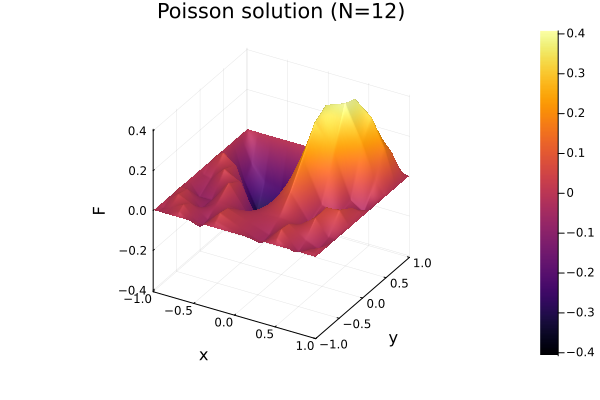
\includegraphics[width=0.48\textwidth]{figures/surface_N12.png}
    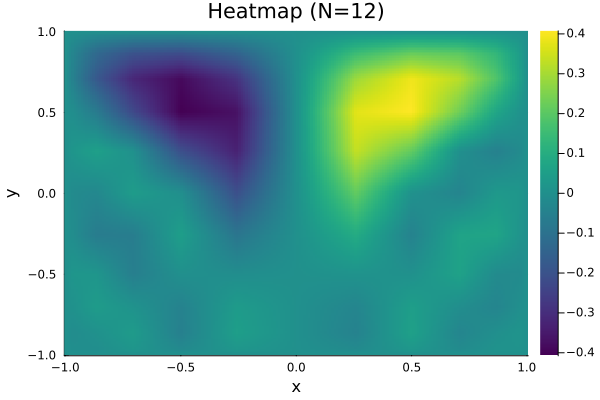
\includegraphics[width=0.48\textwidth]{figures/heatmap_N12.png}\\[4pt]
    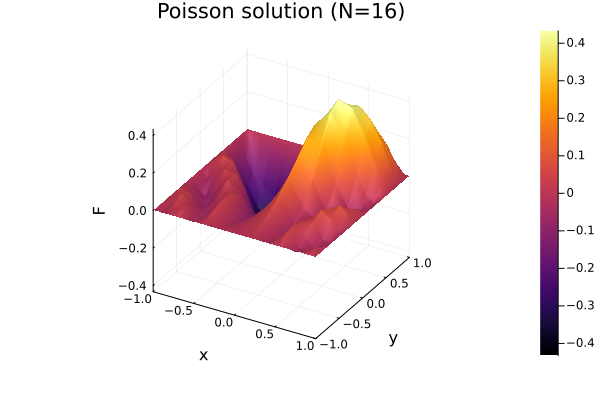
\includegraphics[width=0.48\textwidth]{figures/surface_N16.png}
    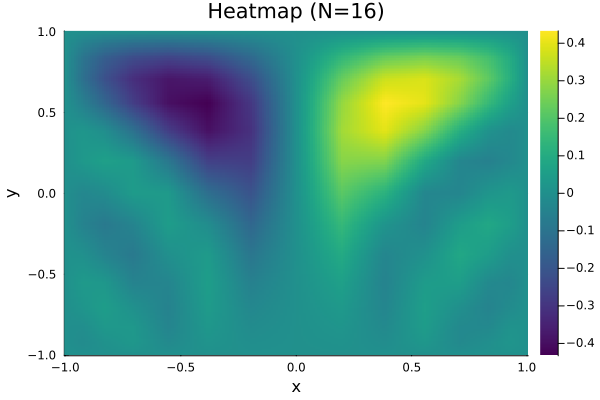
\includegraphics[width=0.48\textwidth]{figures/heatmap_N16.png}\\[4pt]
    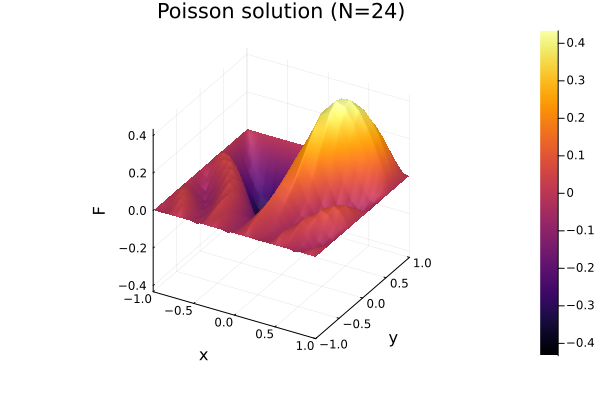
\includegraphics[width=0.48\textwidth]{figures/surface_N24.png}
    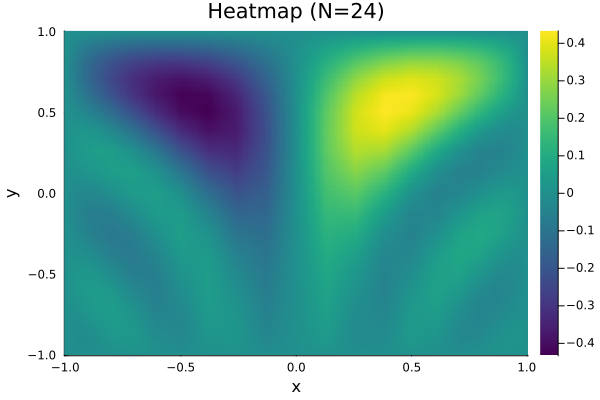
\includegraphics[width=0.48\textwidth]{figures/heatmap_N24.png}\\[4pt]
    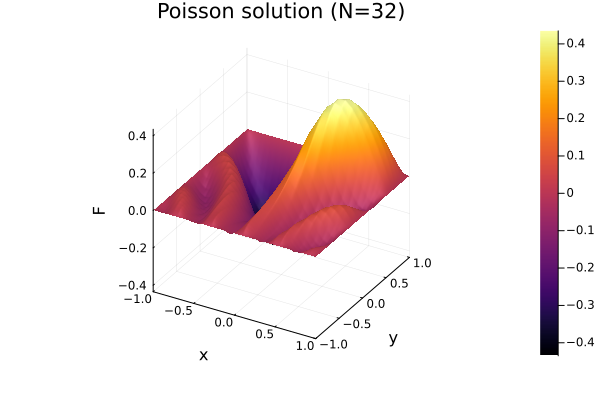
\includegraphics[width=0.48\textwidth]{figures/surface_N32.png}
    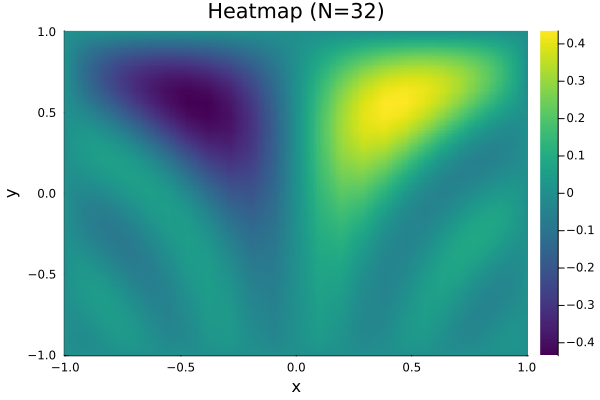
\includegraphics[width=0.48\textwidth]{figures/heatmap_N32.png}\\[4pt]
    \caption{Superfícies e mapas de calor para $N=12$ (linha superior) e $N=32$ (linha inferior). Os demais gráficos seguem o mesmo padrão no diretório \texttt{\_hw9/figures}.}
    \label{fig:poisson_surfaces}
\end{figure}

\section{Setup do Ambiente Julia}

\paragraph{1. Instalação do Julia.}
\begin{enumerate}
    \item Baixe e instale o \texttt{juliaup}, disponível em
    \url{https://github.com/JuliaLang/juliaup}.
    \item Em sistemas Unix, a instalação pode ser feita com:
    \texttt{curl -fsSL https://install.julialang.org | sh}.
    \item Após a instalação, confirme executando \texttt{juliaup status}
    e \texttt{julia +release} (ou a versão específica desejada).
\end{enumerate}

\paragraph{2. Clonar o repositório e ativar o pacote.}
\begin{enumerate}
    \item Clone o repositório oficial:
    \texttt{git clone https://github.com/stealth-lndrs/SpectralTools.git}.
    \item Entre no diretório: \texttt{cd SpectralTools}.
    \item Abra o REPL do Julia: \texttt{julia}.
    \item Ative o projeto: no modo \texttt{pkg} (tecla \texttt{]}), execute
    \texttt{activate .} e depois \texttt{instantiate}.
    \item Para desenvolver o pacote em outro projeto (como o exercício),
    utilize \texttt{pkg> dev /caminho/para/SpectralTools}.
\end{enumerate}

\paragraph{3. Garantir dependências e testes.}
\begin{enumerate}
    \item Ainda no modo \texttt{pkg}, execute \texttt{test} para rodar a suíte
    de testes do pacote e validar a instalação.
    \item Para atualizar dependências, use \texttt{pkg> update}, seguido de
    \texttt{pkg> test}.
    \item Recomenda-se utilizar ambientes dedicados (\texttt{--project=.}) ao
    rodar scripts que dependem do \texttt{SpectralTools}.
\end{enumerate}

Esses passos garantem que qualquer usuário, mesmo sem o Julia previamente
instalado, consiga preparar o ambiente, instalar o pacote do GitHub e
reproduzir os resultados apresentados.


\section{Declaração de uso de LLM}
Foi utilizado um assistente LLM (ChatGPT) para apoiar a organização do relatório, revisão textual e geração de trechos de código e figuras, sempre com validação final do autor.

\end{document}
